\documentclass[border=10pt]{standalone}

\usepackage{tikz}
\usepackage{tikzsymbols}
\usetikzlibrary{calc,patterns,shapes.geometric}

\def\centerarc[#1](#2)(#3:#4:#5){\draw[#1] ($(#2)+({#5*cos(#3)},{#5*sin(#3)})$) arc (#3:#4:#5);}

\begin{document}
	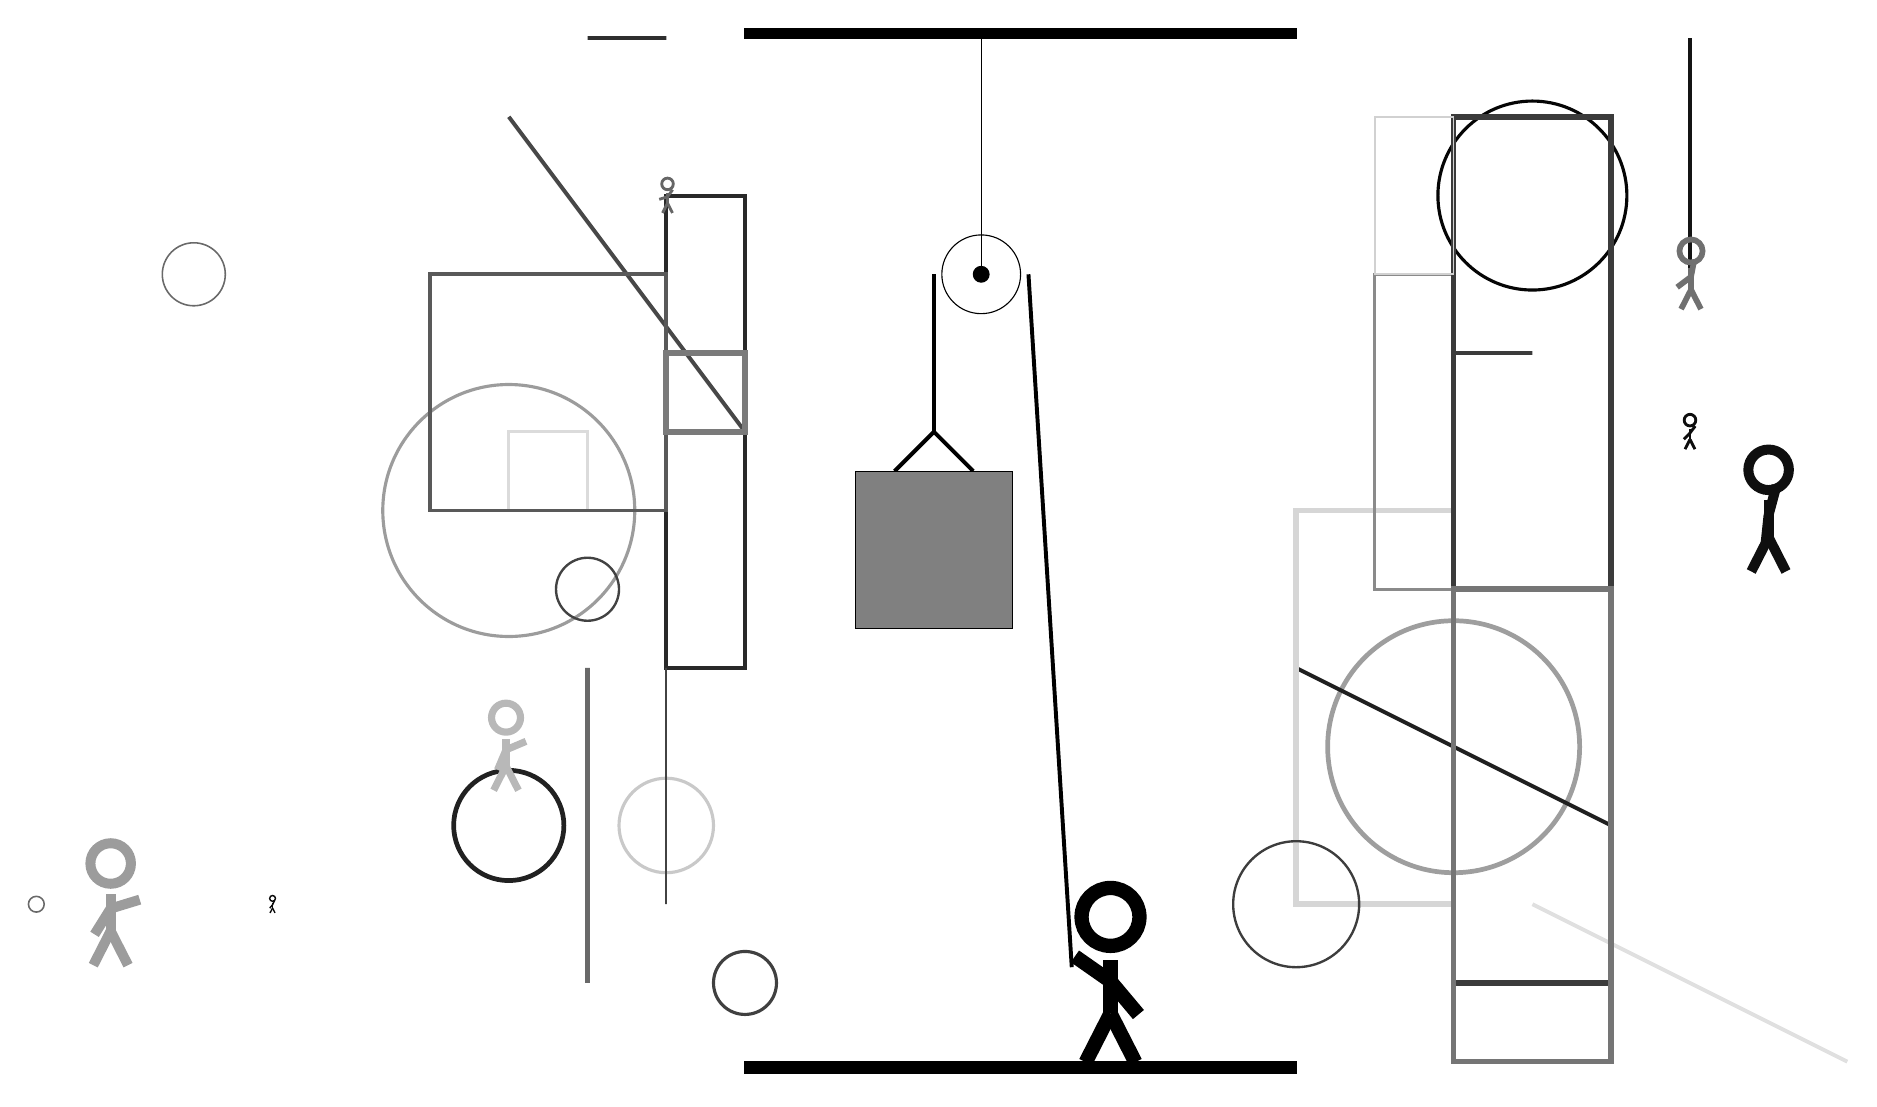
\begin{tikzpicture}
		%%%%% START %%%%%
		
		\draw[fill=black] (-2, 10) rectangle (5, 10.125);
		
		\draw [line width=0.4mm, color=black!39](-5, 4) circle (1.6);
		
		\draw[line width=0.5mm, color=black!12](8, -1) -- (12, -3);
		\draw [line width=0.4mm, color=black!21](-3, 0) circle (0.6);
		\draw[line width=0.5mm, color=black!84] (-2, 8) rectangle (-3, 2);
		\draw[line width=0.6mm, color=black!82] (-4, 10) rectangle (-3, 10);
		\draw [line width=0.3mm, color=black!74](-4, 3) circle (0.4);
		\draw[line width=0.5mm, color=black!77] (7, 6) rectangle (8, 6);
		\draw [line width=0.6mm, color=black!38](7, 1) circle (1.6);
		\draw[line width=0.5mm, color=black!88](9, 0) -- (5, 2);
		
		\draw[line width=0.3mm, color=black!74] (-3, -1) rectangle (-3, 2);
		\draw[line width=0.7mm, color=black!16] (7, -1) rectangle (5, 4);
		\draw[line width=0.4mm, color=black!46] (7, 3) rectangle (6, 7);
		\draw [line width=0.2mm, color=black!59](-11, -1) circle (0.1);
		\draw[line width=0.5mm, color=black!92](10, 7) -- (10, 10);
		\draw [line width=0.4mm, color=black!98](8, 8) circle (1.2);
		\draw[line width=0.5mm, color=black!74](-3, 6) -- (-3, 5);
		\node[line width=0.3mm, color=black!39] at (-10, -1) {\Strichmaxerl[7][58][17]};
		
		\draw[line width=0.4mm, color=black!14] (-4, 4) rectangle (-5, 5);
		\draw[line width=0.5mm, color=black!72](-5, 9) -- (-2, 5);
		\draw [line width=0.6mm, color=black!87](-5, 0) circle (0.7);
		\draw[line width=0.7mm, color=black!77] (7, -2) rectangle (9, 9);
		
		\node[line width=0.4mm, color=black!56] at (10, 7) {\Strichmaxerl[4][37][79]};
		
		\draw[line width=0.6mm, color=black!59] (-4, 2) rectangle (-4, -2);
		\node[line width=0.6mm, color=black!60] at (-3, 8) {\Strichmaxerl[2][17][54]};
		\draw [line width=0.4mm, color=black!75](-2, -2) circle (0.4);
		
		\draw[line width=0.2mm, color=black!18] (7, 7) rectangle (6, 9);
		\draw[line width=0.5mm, color=black!65] (-3, 4) rectangle (-6, 7);
		\node[line width=0.7mm, color=black!96] at (-8, -1) {\Strichmaxerl[1][49][65]};
		
		\node[line width=0.3mm, color=black!28] at (-5, 1) {\Strichmaxerl[5][67][23]};
		\draw[line width=0.7mm, color=black!54] (7, 3) rectangle (9, -3);
		\draw[line width=0.7mm, color=black!52] (-2, 5) rectangle (-3, 6);
		
		\draw [line width=0.3mm, color=black!76](5, -1) circle (0.8);
		\node[line width=0.3mm, color=black!95] at (10, 5) {\Strichmaxerl[2][46][53]};
		\node[line width=0.2mm, color=black!94] at (11, 4) {\Strichmaxerl[7][84][75]};
		\draw [line width=0.2mm, color=black!59](-9, 7) circle (0.4);
		
		\draw (1, 7) circle (0.5);
		\draw[fill=black] (1, 7) circle (0.1);
		\draw (1, 10) -- (1, 7);
		
		\draw[line width=0.5mm] (-0.1, 4.5) -- (0.4, 5.0) -- (0.9, 4.5);
		\draw[fill=black!50] (-0.6, 4.5) rectangle (1.4, 2.5);
		
		\draw[line width=0.5mm] (0.4, 7) -- (0.4, 5.0);
		\centerarc[line width=0.5mm](1, 7)(0:180:0.6);
		\draw[line width=0.5mm](1.6, 7) -- (2.15, -1.8);
		
		\node at (2.6, -1.9) {\Strichmaxerl[10][-35][-50]};
		
		\draw[fill=black] (-2, -3) rectangle (5, -3.15);
		
		%%%%% END %%%%%
	\end{tikzpicture}
\end{document}